\documentclass[sigconf,review,anonymous]{acmart}
%\documentclass[sigconf]{acmart}


% SUBMISSION (double-blind): keep this anonymous line while \documentclass has `anonymous`.
% CAMERA-READY: drop `anonymous` above AND replace this with the real venue/DOI/ISBN from the
% ACM rights email; the real author block below then renders.
\acmConference[Anonymous Review]{Anonymous Review}{2026}{Anonymous}

%\acmYear{2026}
%\copyrightyear{2026}
\acmDOI{}
\acmISBN{}
\pdfmapfile{+libertine.map}
\microtypesetup{expansion=false}
\settopmatter{printacmref=true}
\renewcommand\footnotetextcopyrightpermission[1]{}
\pagestyle{plain}
\emergencystretch=2em
% Tighten float-to-text separation to avoid voids around illustrations
% (placement/spacing only; margins, font, and columns are unchanged).
\setlength{\textfloatsep}{11pt plus 2pt minus 2pt}
\setlength{\intextsep}{9pt plus 2pt minus 2pt}
\setlength{\floatsep}{9pt plus 2pt minus 2pt}
% Discourage widow/orphan lines at column and page breaks.
\widowpenalty=10000
\clubpenalty=10000
\usepackage{pgfplots}
\pgfplotsset{compat=1.18}
\usetikzlibrary{arrows.meta,positioning,fit,backgrounds,calc}
\definecolor{arenaGreen}{HTML}{3D7157}
\definecolor{arenaBlue}{HTML}{466A8D}
\definecolor{arenaRed}{HTML}{A14C5D}
\definecolor{arenaGray}{HTML}{667085}
\definecolor{arenaLight}{HTML}{F5F7FA}
\definecolor{arenaInk}{HTML}{344054}

\title{Auditing AI Investment Recommendations as Executable Actions}

\author{Sidnei Barbieri}
\affiliation{%
  \institution{Aeronautics Institute of Technology}
  \city{São José dos Campos}
  \state{SP}
  \country{Brazil}}
\email{sidneisb@ita.br}

\author{Wellington Vargas}
\affiliation{%
  \institution{Portfel Financial Wealth}
  \city{Barueri}
  \state{SP}
  \country{Brazil}}
\email{wellington.vargas@portfel.com.br}

\author{Ágney Lopes Roth Ferraz}
\affiliation{%
  \institution{Aeronautics Institute of Technology}
  \city{São José dos Campos}
  \state{SP}
  \country{Brazil}}
\email{roth@ita.br}

\begin{abstract}
AI systems increasingly produce investment recommendations, but standard evaluations emphasize realized return or agreement with a reference portfolio. Return is noisy and easy to overfit. Agreement can reward an operationally invalid recommendation. We instead audit each recommendation as an executable financial action before evaluating its return. A deterministic, replayable baseline supports a protocol with three separate measures: validity under portfolio and fee constraints, stability across repeated runs, and agreement with the baseline.

The three measures capture distinct properties. Across a 120-scenario synthetic bank, an agreement-maximizing control reaches $0.86$ agreement and perfect stability while remaining admissible in only $0.58$ of its runs. Exact top-$k$ agreement co-occurs with a violation in $33\%$ of all runs. On an adversarial set, two frontier models are admissible in roughly half of their bare-prompt runs. Disclosing the fee policy produces the largest validity gain, and supplying computed fee arithmetic removes the remaining numeric failures. The baseline therefore serves as a transparent action verifier: its guardrails follow from the fee schedule, its decisions replay from frozen inputs, and the artifact regenerates every reported quantitative result offline.
\end{abstract}

\begin{CCSXML}
<ccs2012> <concept> <concept_id>10010147.10010257</concept_id> <concept_desc>Computing methodologies~Artificial intelligence</concept_desc> <concept_significance>500</concept_significance> </concept> <concept> <concept_id>10002951.10003260.10003309</concept_id> <concept_desc>Information systems~Decision support systems</concept_desc> <concept_significance>300</concept_significance> </concept> <concept> <concept_id>10010405.10010455</concept_id> <concept_desc>Applied computing~Economics</concept_desc> <concept_significance>300</concept_significance> </concept> </ccs2012>
\end{CCSXML}

\ccsdesc[500]{Computing methodologies~Artificial intelligence}
\ccsdesc[300]{Information systems~Decision support systems}
\ccsdesc[300]{Applied computing~Economics}

\keywords{AI in finance, investment recommendations, benchmark, trustworthy AI, reproducibility, transaction costs}

\begin{document}
\maketitle

\section{Introduction}

Large language models (LLMs) now produce investment recommendations, and recent work evaluates them using realized returns or agreement with a reference portfolio \cite{oh2025alpha, spadea2025flarko}. These yardsticks leave an operational gap. Return is noisy and invites overfitting. Agreement rewards a matching recommendation even when it is unusable or unstable. Learned advisors also change under irrelevant inputs and carry latent bias \cite{chawla2025riskadvice, lee2025bias}, properties that return and overlap scores miss.

We evaluate an advisor against a \emph{deterministic, replayable baseline} on three axes: operational \emph{validity} under explicit constraints, \emph{stability} across repeated runs, and \emph{agreement} with the baseline. The baseline is a transparent quality, moat, and compounding policy whose recommendations are pure functions of their inputs. Any run can therefore be replayed and diffed. This design treats the advisor as a candidate generator and subjects its output to a machine-checkable operational contract before measuring return.

The paper makes three contributions. First, it adapts behavioral testing to investment advice through separate measures of validity, stability, and agreement. Deterministic controls and a 120-scenario synthetic benchmark show that reference agreement can coexist with operational failure. Second, it provides a replayable baseline and artifact\footnote{Anonymous reproducibility artifact: \url{https://anonymous.4open.science/r/deterministic-replay-audit/README.md}.}. The fee model is subadditive, the order floor follows from the cost tolerance, and regression tests enforce both properties. Third, it calibrates the baseline against standard allocators. Equal weighting outperforms the tuned weighting, and risk parity nearly matches its Sharpe ratio under walk-forward estimation. These results establish the baseline as a reproducible verifier and show that its specific factor weighting is replaceable.

\section{Related Work}
\label{sec:related}

Factor research supplies established signals for security selection, including gross profitability \cite{novyMarx2013}, quality minus junk \cite{asness2019qmj}, high-dimensional cross-sectional predictors \cite{gu2020machine}, and economic moat \cite{kanuri2016moat}. Our baseline combines quality, moat, and compounding to rank a fixed basket. The audit accepts any deterministic reference policy, and the equal-weight calibration nearly matches the tuned ranking. Signal choice can therefore change the reference picks while leaving the protocol unchanged. The research object is the executability of a recommendation once a candidate set exists.

Classical theory shows that transaction costs induce a \emph{no-trade region}, a band around the target in which the optimal policy holds \cite{constantinides1986capital, davis1990portfolio}. Multiasset extensions derive explicit no-trade geometry \cite{liu2004transaction}, partial adjustment \cite{garleanu2013dynamic}, mixed-integer or convex programs \cite{lobo2007portfolio}, and liquidity or market-impact terms \cite{zhang2019dynamic}. Fixed-fee rebalancing also admits linear-programming and heuristic formulations \cite{delarosa2023planning}. We study recurring small-cash deployment under a quantized step fee. Its economic order floor is the corresponding fixed-cost guardrail.

Language-model portfolio studies reach different conclusions across evaluation windows. Media-driven portfolios report strong short-horizon gains \cite{oh2025alpha}, and knowledge-graph recommenders are scored on behavioral alignment \cite{spadea2025flarko}. A live two-month arena finds gains from short volatility bursts \cite{qian2026ama}. A contamination-free multi-month benchmark finds that most agents trail buy-and-hold and that financial question answering does not transfer to trading skill \cite{chen2025stockbench}. A two-decade evaluation reports weaker performance after removing survivorship, look-ahead, and data-snooping biases \cite{li2026finsaber}.

Despite their different return results, the arena and long-horizon study both attribute behavior mainly to the agent framework and its risk logic \cite{qian2026ama, li2026finsaber}. The emitted action is therefore the useful unit of audit. We evaluate that action at a pre-trade boundary where admissibility is exact and replayable. The calibration backtest applies the same discipline through walk-forward allocator estimation from past-only windows \cite{bailey2014pseudo}. Field evidence provides a compatible operational view: robo-advice can reduce behavioral biases while leaving residual errors \cite{dacunto2019robo}.

Finance trustworthiness benchmarks assess truthfulness, safety, fairness, privacy, and transparency \cite{hu2025fintrust}. PIXIU/FLARE \cite{xie2023pixiu} and FinBen \cite{xie2024finben} cover tasks from sentiment to trading. These benchmarks grade responses or task accuracy, whereas a trade also has portfolio, cash, fee, and grounding constraints. This operational distinction matters because LLM risk assessments shift under irrelevant demographic attributes \cite{chawla2025riskadvice}, investment analyses exhibit confirmation-seeking bias \cite{lee2025bias}, and recommender preferences persist after debiasing \cite{zhi2025productbias}.

Our protocol brings capability-specific behavioral testing \cite{ribeiro2020checklist} and action-level agent evaluation \cite{liu2024agentbench, jimenez2024swebench} to investment recommendations. Each validity rule is a capability test, and the deterministic failure taxonomy is its test matrix. The protocol places an LLM, robo-allocator, or heuristic behind the same interface and measures validity, stability, and agreement against a transparent baseline. Its frozen fact identifiers also provide a verifiable grounding check at the action boundary \cite{ji2023hallucination}.

The verifier also belongs to runtime governance for LLM-generated actions. AgentSpec enforces customizable rules at a pre-execution hook \cite{wang2025agentspec}. VeriGuard synthesizes and verifies policies offline before online validation \cite{miculicich2025veriguard}. ProbGuard predicts violations with probabilistic guarantees \cite{wang2026probguard}, and TRAC monitors temporal compliance \cite{alamdari2026formalmethods}. Our verifier uses a hand-specified financial contract over declared quantities, yielding exact and replayable verdicts. The evaluation adds empirical evidence that agreement and admissibility diverge on frontier models, that contract disclosure changes validity, and that supplied arithmetic removes numeric failures.

Backtest overfitting is easy to produce and hard to detect \cite{bailey2014pseudo}, while naive $1/N$ diversification remains a strong baseline \cite{demiguel2009naive}. We therefore regenerate every empirical figure from a deterministic engine and report the calibration when simple allocators outperform the tuned weighting.

\section{Artifact and Audit Protocol}
\label{sec:audit}

\begin{figure*}[t]
  \centering
  \resizebox{0.86\textwidth}{!}{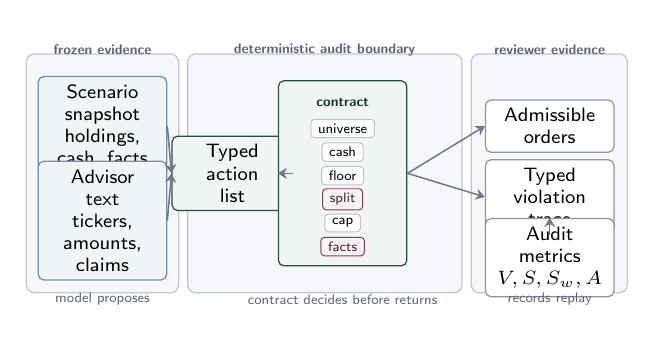
\begin{tikzpicture}[
  x=1cm,
  y=1cm,
  >=Stealth,
  zone/.style={
    rounded corners=3pt,
    draw=arenaGray!40,
    fill=arenaLight,
    line width=.45pt
  },
  zonelabel/.style={
    font=\sffamily\tiny\bfseries,
    text=arenaGray!90!black,
    align=center
  },
  card/.style={
    rounded corners=2pt,
    draw=arenaInk!50,
    fill=white,
    line width=.45pt,
    align=center,
    inner xsep=4pt,
    inner ysep=3pt,
    font=\sffamily\scriptsize
  },
  inputcard/.style={card, draw=arenaBlue!75, fill=arenaBlue!7},
  typedcard/.style={card, draw=arenaGreen!70!black, fill=arenaGreen!7},
  verdictcard/.style={card, draw=arenaInk!55, fill=white},
  rulechip/.style={
    rounded corners=1.3pt,
    draw=arenaInk!32,
    fill=white,
    line width=.35pt,
    font=\sffamily\tiny,
    inner xsep=2.6pt,
    inner ysep=1.6pt
  },
  riskchip/.style={
    rulechip,
    draw=arenaRed!80!black,
    fill=arenaRed!7,
    text=arenaRed!45!black
  },
  flow/.style={-{Stealth[length=3.3pt,width=4pt]}, draw=arenaInk!70, line width=.55pt},
  softflow/.style={flow, dashed, draw=arenaGray!75},
  note/.style={font=\sffamily\tiny, text=arenaGray!90!black, align=center}
]

\path[use as bounding box] (-.15,-1.8) rectangle (7.45,1.9);

\begin{scope}[on background layer]
  \node[zone, fit={(-.05,-1.35) (1.65,1.45)}] (zinput) {};
  \node[zone, fit={(2.0,-1.35) (5.25,1.45)}] (zcontract) {};
  \node[zone, fit={(5.6,-1.35) (7.35,1.45)}] (zout) {};
\end{scope}

\node[zonelabel] at (.8,1.62) {frozen evidence};
\node[zonelabel] at (3.62,1.62) {deterministic audit boundary};
\node[zonelabel] at (6.48,1.62) {reviewer evidence};

\node[inputcard, text width=1.35cm] (scenario) at (.8,.65)
  {Scenario\\snapshot\\\scriptsize holdings, cash, facts};
\node[inputcard, text width=1.35cm] (advisor) at (.8,-.55)
  {Advisor\\text\\\scriptsize tickers, amounts, claims};

\node[typedcard, text width=1.25cm] (action) at (2.45,.05)
  {Typed\\action\\list};
\node[typedcard, text width=1.35cm, minimum height=2.35cm] (contract) at (3.85,.05)
  {};
\node[zonelabel, text=arenaGreen!45!black] at (3.85,.95) {contract};

\node[rulechip] at (3.85,.62) {universe};
\node[rulechip] at (3.85,.32) {cash};
\node[rulechip] at (3.85,.02) {floor};
\node[riskchip] at (3.85,-.28) {split};
\node[rulechip] at (3.85,-.58) {cap};
\node[riskchip] at (3.85,-.88) {facts};

\node[verdictcard, text width=1.35cm] (orders) at (6.48,.65)
  {Admissible\\orders};
\node[verdictcard, text width=1.35cm] (trace) at (6.48,-.25)
  {Typed\\violation\\trace};
\node[verdictcard, text width=1.35cm] (metrics) at (6.48,-1.02)
  {Audit\\metrics\\\scriptsize $V,S,S_w,A$};

\draw[flow] (scenario.east) -- (action.west);
\draw[flow] (advisor.east) -- (action.west);
\draw[flow] (action.east) -- (contract.west);
\draw[flow] (contract.east) -- (orders.west);
\draw[flow] (contract.east) -- (trace.west);
\draw[flow] (trace.south) -- (metrics.north);

\node[note] at (.8,-1.55) {model proposes};
\node[note] at (3.85,-1.55) {contract decides before returns};
\node[note] at (6.48,-1.55) {records replay};
\end{tikzpicture}
}
\caption{The audit boundary turns advisor text into executable orders and typed violations before any return is computed.}
\Description{A mechanism diagram showing frozen scenario data and advisor output entering a normalizer and deterministic verifier, which applies policy rules and emits admissible orders, violation traces, and audit metrics.}
  \label{fig:workflow}
\end{figure*}

The backend separates API data-transfer objects, portfolio importers, provider adapters, analytics scoring, and deployment planning. Network access is isolated behind provider abstractions. The scoring and deployment modules perform no I/O: a recommendation is a pure function of the tuple.
\[
(\text{holdings},\ \text{fundamentals},\ \text{cash},\ \text{policy version}).
\]
Referential transparency supports every reported quantitative result. The reviewer path runs \texttt{run\_experiments.py} for the experiment JSON and empirical figures, \texttt{run\_ai\_advisor\_audit.py} for the advisor-audit panel, and \texttt{collect\_advisor\_runs.py} for the frontier-model audit. These drivers use frozen data and explicit state. A replay test feeds the same input tuple twice and requires byte-identical orders, exclusions, and rankings. The engine draws no random numbers and breaks ties by ticker. Fees and the order floor use integer tranche counts, validity and agreement use set membership, and stability uses ratios of those sets. This representation prevents floating-point noise from changing a verdict. Figure~\ref{fig:workflow} shows the boundary: the model proposes text, and deterministic code emits executable orders or typed violations.

The composite score is the bounded linear functional $s=w_m\,\mathrm{moat}+w_c\,\mathrm{comp}+w_v\,\mathrm{val}$, with sub-scores in $[0,100]$ and weights $(w_m,w_c,w_v)=(0.40,0.35,0.25)$. The planner excludes holdings above $1.3\times$ equal weight and themes at their concentration cap. It then ranks the remaining candidates by $s$ and sizes orders against available cash.

We score an advisor on three axes. A \emph{scenario} fixes current holdings, available cash, an allowed universe, per-scenario constraints, and the baseline recommendation. The constraints include a recommendation cap, add-only or trim rules, concentration exclusions, and the economic order floor from Section~\ref{sec:guardrail}. The advisor returns tickers, optional dollar amounts, and cited facts. \emph{Validity} is the fraction of runs that satisfy every constraint. \emph{Stability} is the mean pairwise overlap across repeated recommendations, augmented by an amount-aware score when the output includes allocations. \emph{Agreement} is overlap with the baseline's funded top-$k$ set, where the scenario's cash and recommendation cap determine $k$. Agreement is descriptive because disagreement may represent either useful novelty or error. Changing $k$, or replacing overlap with rank correlation, rescales agreement while leaving validity and stability unchanged.

The validity checks form a deterministic failure taxonomy (Table~\ref{tab:taxonomy}). Each category is an exact test on the advisor output and frozen scenario, so every failed run has a named cause. The sub-tranche control triggers the fee-worsening split, a regression test triggers the frozen concentration predicate, and the fact-hallucination control triggers the ungrounded-fact predicate.

\begin{table}[tb]
\caption{Deterministic failure taxonomy: each category is an exact test on advisor output and the frozen scenario ($a_i$ is leg $i$'s amount, $T$ the fee tranche, $c/\tau$ the economic floor).}
  \label{tab:taxonomy}
\begin{tabular}{ll}
\toprule
Failure & Deterministic test \\
\midrule
Out-of-universe ticker & ticker $\notin$ allowed set \\
Recommendation-cap breach & count $>$ cap \\
Already-owned (add-only) & ticker $\in$ held set \\
Cash overrun & $\textstyle\sum_i a_i >$ cash \\
Below-floor order & $a_i < c/\tau$ \\
Fee-worsening split & $\textstyle\sum_i \lceil a_i/T\rceil > \lceil (\textstyle\sum_i a_i)/T\rceil$ \\
Concentration breach & ticker $\in$ frozen over-cap set \\
Ungrounded cited fact & fact id $\notin$ scenario set \\
\bottomrule
  \end{tabular}
\end{table}

A single trace illustrates the mechanism. In the sub-tranche scenario, the advisor has \$900 to deploy under a \$2.50 fee per \$1{,}000 tranche. One \$900 order pays one tranche fee and is admissible. A bare model splits the cash into two \$450 legs. The verifier applies the split rule from Table~\ref{tab:taxonomy}: $\lceil 450/1000\rceil + \lceil 450/1000\rceil = 2 > 1 = \lceil 900/1000\rceil$. It returns a fee-worsening split before observing any price. The logged inputs now reproduce a typed action and an exact verdict.

Seven constructed archetype controls show that the three axes are independent (Figure~\ref{fig:audit}). The naive diversifier agrees with the baseline and is perfectly stable, yet violates the fee rule by splitting sub-tranche cash. A second control is valid and stable with zero agreement. An overlap-only benchmark ranks the invalid diversifier above the admissible alternative.

For an advisor that returns ticker sets $r_1,\dots,r_n$ over repeated runs of a scenario with baseline top-$k$ set $b$, the metrics are:
\[
  \begin{array}{r@{\;=\;}l@{\qquad}r@{\;=\;}l}
V & \tfrac1n\sum_j \mathbf{1}[\mathrm{viol}(r_j)=\varnothing] & S & \dbinom{n}{2}^{-1}\!\sum_{i<j} J(r_i,r_j) \\[1.8ex] S_w & 1 - \dbinom{n}{2}^{-1}\!\sum_{i<j} \mathrm{TV}(w_i,w_j) & A & \tfrac1n\sum_j \dfrac{|r_j\cap b|}{k}
  \end{array}
\]

\begin{figure}[tb]
  \centering
  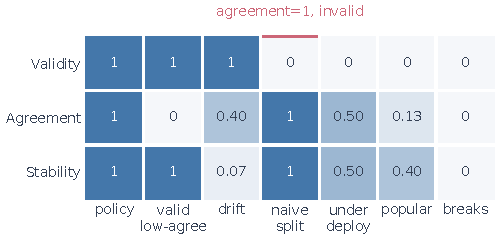
\includegraphics[width=\columnwidth]{figures/ai_advisor_audit.pdf}
  \caption{The archetype controls separate validity, agreement, and stability.}
\Description{Heat-map matrix of validity, agreement, and stability across seven advisor archetypes, showing that high agreement does not coincide with high validity.}
  \label{fig:audit}
\end{figure}
where $J$ is Jaccard overlap, $\mathrm{viol}$ is the constraint set of $r_j$, $w_j$ normalizes run $j$'s dollar amounts to weights, and $\mathrm{TV}$ is total-variation distance. When the baseline funds no position ($k=0$), agreement is 1 only when the advisor also holds no position. The sizing stability $S_w\in[0,1]$ is reported when a scenario requires amounts. Once advisor outputs are frozen, the audit replays process quality before performance statistics are computed.

The controls also justify the sizing axis. In the sub-tranche scenario, the naive diversifier repeats the same tickers on every run and reaches set stability $1.0$. Its changing dollar split lowers $S_w$ to $0.93$, and an under-deploying control reaches $S_w=0.33$. The deterministic policy holds both terms at $1.0$. The amount-aware term therefore exposes sizing drift hidden by set overlap.

The audit then scores frozen outputs from GPT-5.5 (OpenAI) and Opus-4.8 (Anthropic) under the shared configuration in Table~\ref{tab:fairness}: single-message JSON-only calls, temperature $1.0$, no tools, and no system prompt. Each hashed record contains the provider, model label, prompt, prompt hash, raw and parsed response, token usage, finish reason, latency, and timestamp. A pilot with a $500$-token budget truncated the reasoning model and produced an apparent abstention. We raised the completion budget and added a per-run truncation flag before freezing the reported campaign. Every reported run has $\textit{truncated}=0$.

We sweep 24 adversarial scenarios across three prompt arms with five runs each. A global random order distributes all $720$ cells across the frozen campaign, reducing alignment between an arm and temporal or model-version drift. Cash values straddle fee tranches, and the scenario facts omit the fee. The \emph{bare} arm supplies the task and schema. The \emph{policy} arm adds the fee schedule, \$250 floor, and fee-neutral-split rule. The \emph{scaffold} arm also supplies the scenario's computed one- and two-order fees.

Bare validity is $0.59$ for GPT-5.5 and $0.51$ for Opus-4.8. Scenario-clustered bootstrap $95\%$ intervals are $[0.38,0.79]$ and $[0.30,0.71]$ from $2{,}000$ resamples of the 24 scenarios. GPT-5.5 produces $49$ fee-worsening splits and $29$ below-floor orders, while Opus-4.8 omits required amounts on $52$ runs. Policy disclosure raises validity to $0.98$ and $0.93$, with intervals $[0.95,1.00]$ and $[0.83,1.00]$. The remaining numeric failures are two and eight fee-worsening splits. The scaffold eliminates those splits and reaches $1.00$ and $0.97$. Its four residual failures are already-owned recommendations from Opus-4.8. The policy intervals are separated from their bare counterparts, while the policy-to-scaffold difference remains within bootstrap noise. Contract disclosure produces the main gain, supplied arithmetic removes the numeric residue, and the verifier identifies the remaining semantic error.

\begin{table}[tb]
\caption{Shared frontier-model configuration.}
  \label{tab:fairness}
\begin{tabular}{ll}
\toprule
Parameter & Value (both models) \\
\midrule
Temperature & $1.0$ (provider default) \\
Completion budget & $4000$ tokens \\
Top-$p$ & provider default \\
Tools / system prompt & none \\
Runs per scenario & $5$ \\
Truncated completions & $0$ \\
\bottomrule
  \end{tabular}
\end{table}

The offline scenario bank tests the same separation at scale. It contains 120 frozen scenarios, with ten variants in each of twelve categories spanning cash deployment, ownership, fee sensitivity, grounding, drawdowns, and rebalancing. Dated fact identifiers cover returns, rates, employment, and concentration claims, making grounding a deterministic set check over realistic inputs. The manifest freezes cash, allowed tickers, baseline tickers, fact IDs, and constraints before scoring. Five constructed advisors run five times per scenario, yielding 3,000 replayed outputs. They implement the contract, maximize agreement while splitting orders, change tickers across runs, cite unsupported facts, or overspend cash. This bank isolates metric behavior under controlled stressors. The 24-scenario campaign above provides the frontier-model evidence.

\begin{table}[tb]
\caption{Frozen scenario-bank results over 120 scenarios and 3,000 advisor outputs. High agreement and stability do not imply validity.}
  \label{tab:scenario-bank}
\begin{tabular}{lrrrr}
\toprule
Advisor & Valid & Agree & Set $S$ & Agr.-FP \\
\midrule
Contract & $1.00$ & $0.92$ & $1.00$ & $0.00$ \\
Agreement split & $0.58$ & $0.86$ & $1.00$ & $0.33$ \\
Unstable selector & $0.88$ & $0.28$ & $0.13$ & $0.00$ \\
Fact hallucination & $0.00$ & $0.83$ & $1.00$ & $0.75$ \\
Cash overrun & $0.50$ & $0.60$ & $1.00$ & $0.33$ \\
\bottomrule
  \end{tabular}
\end{table}

Table~\ref{tab:scenario-bank} reports the bank results. The agreement-only false-positive rate (Agr.-FP) is the fraction of runs that reproduce the funded top-$k$ set while violating a constraint. For the agreement splitter, this occurs in $33\%$ of all runs despite $0.86$ agreement and perfect stability. The fact-hallucination stressor maintains $0.83$ agreement and perfect stability while violating grounding on every run. Across the bank, the taxonomy records 600 ungrounded facts, 300 cash overruns, 150 fee-worsening splits, 150 recommendation-cap violations, 120 malformed amount outputs, and 100 below-floor orders. The hashed manifest versions the balanced design of ten variants for each of twelve categories.

\section{Deterministic Verification}
\label{sec:portfolio-verification}
\label{sec:fees}
\label{sec:guardrail}

The audit protocol assigns the advisor to generate candidates and the deterministic layer to select an executable action. A ticker can rank highly in isolation yet remain unsuitable for the current portfolio because it increases concentration, consumes cash inefficiently, or repeats a full exposure. The verifier evaluates each candidate in portfolio context.

The verifier uses current holdings, themes, cash, fees, and candidate scores. It projects the theme weight of a starter position, assigns a structural role (diversifier, theme reinforcement, or concentration watch), and ranks each candidate by portfolio fit. In the artifact's controlled scenario, the highest-quality Platforms name (quality $90$) would raise an already-crowded theme from $23.0\%$ to $30.7\%$. The verifier instead selects an Industrial diversifier (quality $84$) at a new $10.0\%$ exposure over a Healthcare name (quality $82$) that reinforces an existing $14.5\%$ theme. Isolated ranking selects Platforms. Portfolio verification selects Industrial.

This separation is the central design move. The learned system searches a large, noisy space of plausible investment theses. The deterministic artifact checks the proposed action against a compact, replayable admissibility contract.

Every contract threshold is tied to a declared quantity. Before evaluation, the scenario derives the candidates whose projected position exceeds $1.3\times$ the equal-weight share or whose theme exceeds the $20\%$ exposure cap. Selecting any such candidate violates the contract. Orders must also reach the economic floor $c/\tau$, splits must be fee-neutral against the consolidated order, and cited facts must belong to the scenario snapshot. The position and theme bounds use a ratio of equal weight and a single cap, allowing the same contract to apply to any basket. A versioned ticker-to-theme map fixes theme membership and is logged with the scenario. A finite set of fact identifiers makes grounding an exact membership test.

The same verifier must translate a ranking into executable orders. That translation matters whenever the broker charges a fixed cost $c$ for each started tranche of size $T$ in a single-symbol order:
\begin{equation}
f(a) = \left\lceil \tfrac{a}{T} \right\rceil c,
  \qquad T = \$1000,\ c = \$2.50.
  \label{eq:fee}
\end{equation}
The ceiling creates discrete fee jumps. A \$1{,}001 order pays two tranches, the same as a \$2{,}000 order. Subadditivity, $f(a+b)\le f(a)+f(b)$, means that splitting cash across symbols preserves or increases the fee.

We measure the excess fee from splitting as a diversification premium,
\begin{equation}
\pi(a_1,\dots,a_k) = \sum_i f(a_i) - f\!\Big(\sum_i a_i\Big) \;\ge\; 0,
  \label{eq:premium}
\end{equation}
where the right-hand term is the cost reference for one order of the same size. A positive premium measures the implementation cost of diversification.

We swept cash from \$250 to \$5000 and compared three policies against the single-order lower bound: a \emph{naive} split strictly proportional to score, a \emph{fee-aware} planner, and (as a reference) the single order. Naive splitting incurs $\pi=\$2.50$ in recurring bands wherever the two legs cross an extra tranche boundary (Figure~\ref{fig:premium}).

\begin{figure}[tb]
  \centering
  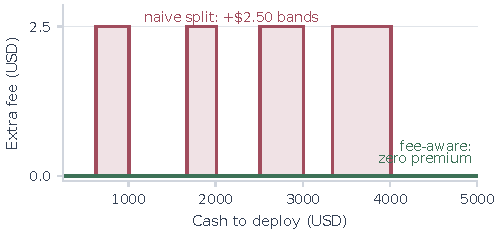
\includegraphics[width=\columnwidth]{figures/fee_premium.pdf}
\caption{Naive splitting pays recurring fee premiums. The fee-aware planner stays on the zero-premium frontier.}
\Description{Line chart showing naive split fee premiums above zero in repeated bands, while the fee-aware planner remains at zero premium.}
  \label{fig:premium}
\end{figure}

The sweep exposed and fixed a planner defect. A score-proportional split can pay an extra \$2.50 when two sub-tranche legs each start a fee unit. The earlier planner made that mistake for cash between \$625 and \$1000 under a 60/40 split. The corrected planner diversifies when the split is fee-neutral and consolidates otherwise. A property test asserts that its fee never exceeds the single-order lower bound across the cash grid.

A second cost rule prevents tiny orders. If a trade should lose at most a fraction $\tau$ to the fixed fee, then the binding first-tranche order is
\begin{equation}
  \mathrm{MIN} = \frac{c}{\tau} = \frac{\$2.50}{0.01} = \$250,
  \label{eq:min}
\end{equation}
Below this floor, the planner holds cash, and a second economic order requires \$500. At 1\% tolerance, flat fees of \$1, \$5, and \$9.99 imply floors of \$100, \$500, and \$999. Zero commission yields a zero floor. For started tranches, a finite floor exists when $c/T\leq\tau$. Then $c/\tau\leq T$, so the binding floor lies in the first tranche. The guardrail follows directly from the fee schedule.

We compare the planner with the consolidated-fee lower bound and a deployment MIP. The MIP maximizes $\sum_i x_i$ under $\sum_i x_i\leq\mathrm{cash}$, $x_i=0$ unless order flag $z_i=1$, and $x_i\ge(c/\tau)z_i$. Because it omits portfolio limits, its PuLP/CBC solution upper-bounds feasible deployment under the full contract.

Across \$250--\$5{,}000, where portfolio limits do not bind, the planner reaches both bounds: the deployment gap and fee premium are zero. This establishes exactness in the studied nonbinding regime. Elsewhere, the MIP remains an upper bound.

\section{Calibrating the Baseline}
\label{sec:weighting}

This section calibrates the audit's reference policy and tests whether its factor weighting materially determines the result. Because the composite score is linear, zeroing a weight isolates one factor, and per-position sub-scores allow recomposition without re-fetching data.

On a fixed basket with deterministic synthetic fundamentals, we recomposed the ranking under single-factor and equal weights. We measured Spearman correlation with the baseline ordering and churn in the funded top-2 (Figure~\ref{fig:ablation}). Single factors reorder the basket sharply. Moat-only and valuation-only are anti-correlated with the baseline, whereas equal thirds reproduce it almost exactly ($\rho=0.97$, zero churn). The funded picks remain stable under $\pm10\%$ weight perturbation.

\begin{figure}[tb]
  \centering
  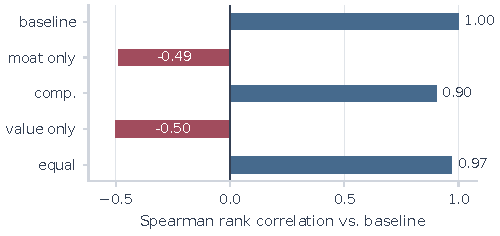
\includegraphics[width=\columnwidth]{figures/ablation.pdf}
\caption{Each factor reshapes the ranking differently. Equal weighting tracks the tuned baseline.}
\Description{Horizontal bar chart comparing Spearman rank correlation against the baseline across moat-only, compounding-only, valuation-only, equal-thirds, and baseline weighting schemes.}
  \label{fig:ablation}
\end{figure}

We backtested the 17-name basket over 2021-01-05 to 2026-06-04 (1360 trading days) using free adjusted closes (Table~\ref{tab:backtest}). The comparison includes market-value current weighting, equal weighting, long-only minimum variance, and equal-risk-contribution risk parity. Allocator weights are estimated walk-forward from a rolling 252-day return window with a 20\% constant-variance shrinkage target, 63-day rebalancing, and a 10 bp turnover cost. The allocator uses equal weights until 63 observations exist. Minimum variance uses an active-set reduction on the closed-form solution, and risk parity uses the Maillard fixed-point iteration.

The score-weighted basket exceeds SPY by $4.96$ percentage points in compound annual growth rate (CAGR) and $0.18$ in Sharpe ratio. Equal weighting is stronger at $22.8\%$ CAGR and $1.19$ Sharpe ratio. The walk-forward risk-parity baseline approaches the score-weighted Sharpe ($1.11$ versus $1.14$ after rounding) with lower return. Minimum variance has the shallowest drawdown ($-21.7\%$). Periodic rebalancing reduces CAGR from $20.7\%$ to $18.8\%$ despite low explicit cost. Together, the ablation and backtest show that factor weighting is a replaceable component of the verifier.

\begin{table}[tb]
\caption{Current-basket backtest, 2021-01-05 to 2026-06-04 (1360 days), buy and hold unless noted. Allocator baselines are walk-forward with shrinkage and turnover cost.}
  \label{tab:backtest}
\begin{tabular}{lrrr}
\toprule
Strategy & CAGR & Sharpe & Max DD \\
\midrule
Equal weight & $22.8\%$ & $\mathbf{1.19}$ & $-27.1\%$ \\
Current weight (ours) & $20.7\%$ & $1.14$ & $-26.8\%$ \\
Risk parity & $18.8\%$ & $1.11$ & $-26.4\%$ \\
Minimum variance & $14.1\%$ & $0.94$ & $\mathbf{-21.7\%}$ \\
Benchmark (SPY) & $15.8\%$ & $0.95$ & $-24.5\%$ \\
\midrule
Rebalanced current & $18.8\%$ & $1.09$ & $-28.0\%$ \\
\bottomrule
  \end{tabular}
\end{table}

\begin{figure}[tb]
  \centering
  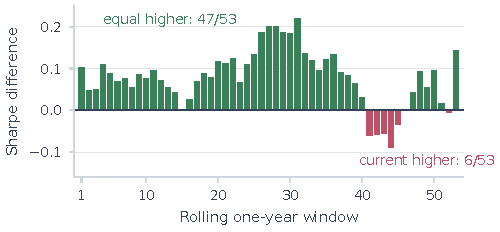
\includegraphics[width=\columnwidth]{figures/robustness.pdf}
  \caption{Rolling one-year excess Sharpe often favors equal weighting.}
\Description{Bar chart of the rolling one-year Sharpe difference between equal and current weighting across 53 windows, positive in most windows but with several negative stretches.}
  \label{fig:robustness}
\end{figure}

We probe the equal-versus-current result over the same daily-return matrix using fixed-weight, daily-rebalanced portfolios. In rolling one-year windows stepped monthly, equal weighting has the higher Sharpe in $37$ of $53$ windows ($70\%$; Figure~\ref{fig:robustness}). The negative windows cluster in a few stretches. A circular block bootstrap ($2{,}000$ resamples of 21-day blocks, fixed seed) gives a full-period Sharpe difference $\mathrm{Sharpe}(\text{equal})-\mathrm{Sharpe}(\text{current})$ of $+0.053$, a $95\%$ interval of $[-0.024, +0.127]$, and $P(\text{equal better})=91\%$. The interval includes zero, so the experiment measures no advantage over the parameter-free control at the $5\%$ level. This result confirms that the verifier does not depend on the tuned weighting.

\section{Discussion}

The benchmark makes one claim: whether an action is admissible, grounded, stable, and reproducible before any return is computed. That is the operational boundary that return-based and overlap-based benchmarks lack. Any advisor runs behind the same interface and answers one question: given these dated facts, this portfolio, and this cost model, did it emit a valid, stable, grounded, portfolio-admissible action? The question is small enough to answer exactly and important enough to ask before any performance claim.

The controls establish a precise result: validity, stability, and agreement are separable. A constructed advisor that agrees with the baseline yet violates a constraint is an existence proof that the three axes measure different things, which a single conflated score cannot represent. The bank quantifies that separation at scale, and the model audit shows that contract disclosure and computed arithmetic remove distinct layers of failure. Separability is the property that an action-level benchmark must report, and it is established by construction rather than estimated as a failure rate.

Live arenas and bias-mitigated long-horizon backtests reach different return conclusions but agree that agent decision and risk logic drive behavior more than the model backbone. The verifier externalizes that logic as an explicit admissibility layer. It shifts evaluation from the model family to the emitted action and yields stable, replayable verdicts across horizons and regimes.

The empirical calibration sharpens the claim. In fee-quantized markets, diversification incurs an implementation cost, so the planner diversifies only when the split is fee-neutral. The fundamentals-weighted basket beats the market benchmark but ranks third of five on risk-adjusted return, behind equal weighting and risk parity. This result is consistent with the difficulty of beating $1/N$ diversification \cite{demiguel2009naive} and reinforces the verifier's modular design: reference weighting can change without changing the admissibility contract.

The protocol scores operational requirements directly: advice must be executable, repeatable, grounded in the frozen scenario, and compatible with portfolio constraints. An advisor that eliminates cash overruns and sub-tranche splits improves on requirements that the system must satisfy in deployment. Validity alone still admits a trivial always-hold policy, so agreement and return remain companion measures. Admissibility serves as the pre-filter for those outcome measures.

The frontier-model audit identifies two failure layers. Bare prompts leave both models admissible in roughly half of the runs. Declaring the contract raises validity to $0.98$ and $0.93$, and supplying computed fee arithmetic removes the remaining numeric failures. The bare arm measures behavior under an undisclosed contract. Contract disclosure and arithmetic scaffolding address specification and computation failures, respectively. The controls and scenario bank reproduce the same separation, with high agreement despite invalid actions.

The evidence scope is explicit. The backtest calibrates a current basket on free adjusted closes and does not evaluate point-in-time security selection. The cost model covers fixed per-order tranche fees. Spreads, taxes, slippage, and integer lots remain outside the evaluated contract.

\paragraph{Modular governance contracts.} The contract is a set of decidable predicates $C=\{p_1,\dots,p_n\}$ over a scenario $\sigma$ and proposed action $a$. The verdict $v=\mathrm{evaluate}(C,\sigma,a)$ admits $a$ iff every predicate holds. An integer-share predicate requires $a_i/p_i\in\mathbb{Z}$, a spread budget bounds $s_i a_i$, a liquidity cap limits order size relative to frozen volume, and restricted-list and sector predicates constrain eligible assets. A different commission or odd-lot schedule replaces the fee predicate. Its economic floor becomes $\inf\{a>0:f(a)/a\leq\tau\}$, and consolidation remains a lower bound when the new $f$ is subadditive. The artifact includes restricted-list and frozen concentration-block predicates with regression tests. More frozen scenarios widen coverage, while more predicates widen governance. Both extensions preserve the protocol, replay mechanism, and evaluation metrics. This structure gives heterogeneous advisors a shared scenario bank, a declarative contract, and decision records that serve as a compliance audit trail.

Portfolio systems already perform proprietary pre-trade checks. This protocol turns that layer into a shared, declarative, model-agnostic benchmark. Identical frozen scenarios and one admissibility contract score every advisor on the same terms, with each rejection recorded as a typed, replayable reason.

\section{Conclusion}

Admissibility is an independent property of an AI-generated action, separable from agreement and return. On real frontier models, declaring the contract produces the largest validity gain, while deterministic arithmetic removes the remaining numeric failures. Auditing a recommendation before any price path is realized turns vague trust into a typed, replayable verdict. We release a deterministic baseline, protocol, and frozen scenario bank that judges any advisor on identical terms and accepts richer microstructure or compliance rules as additional predicates without changing the score.

\section*{LLM usage considerations}
The authors used Grammarly, ChatGPT, Claude, and Codex for grammar and editorial revision, code review and refactoring, test generation, and figure formatting. The authors designed the study and protocol, reviewed and executed the code, verified all experimental outputs and references, and take responsibility for the complete work.

\bibliographystyle{ACM-Reference-Format}
\bibliography{references}

\end{document}
